% !TEX root = ../presentation.tex
% !BIB program = biber
% !TEX program = xelatex

\section{Introduction}


\begin{frame}
    \frametitle{Healthcare}
    \begin{quotation}
        \noindent\centering
        Healthcare is the improvement of health via the {\color{dtured}prevention}, {\color{dtured}diagnosis}, {\color{dtured}treatment}, {\color{dtured}amelioration} or {\color{dtured}cure} of {\color{theme-green}disease}, {\color{theme-green}illness}, {\color{theme-green}injury}, and {\color{theme-green}other physical and mental impairments} in people.
    \end{quotation}
\end{frame}


\begin{frame}
    \frametitle{Medical dialogue}
    \begin{figure}
        \centering
        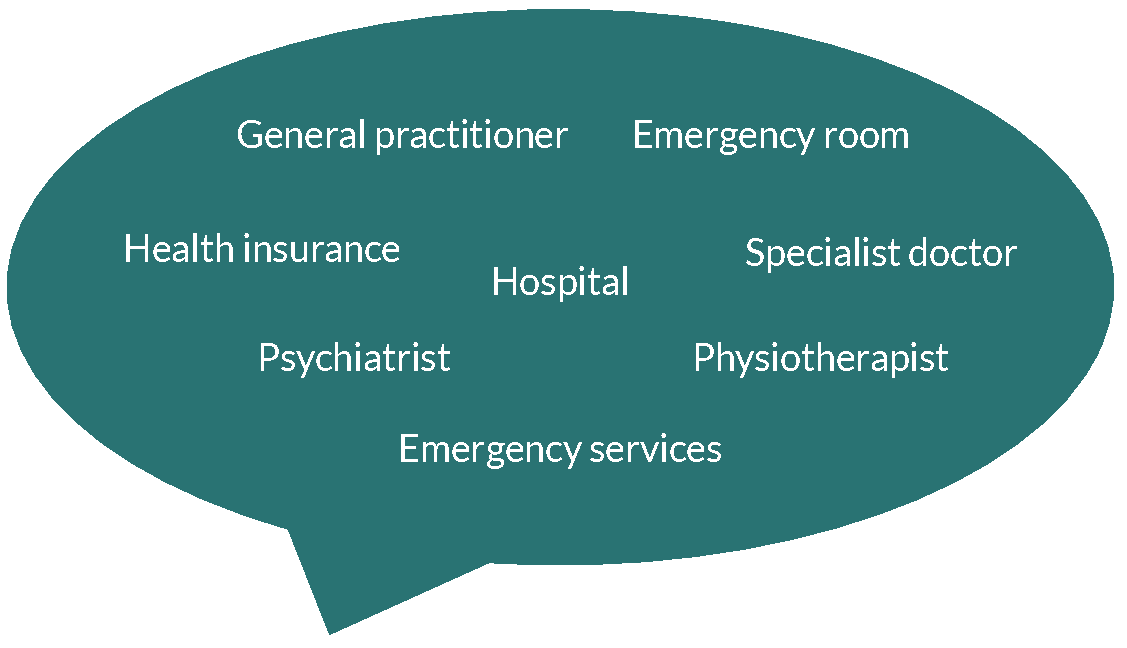
\includegraphics[width=0.7\paperwidth]{figures/speech_bubble.pdf}
    \end{figure}

    \note[item]{}
\end{frame}


\begin{frame}
    \frametitle{Medical dialogue}
    \begin{enumerate}
        \item Failure of communication is a leading cause of medical error contributing to two out of three adverse events \cite{starmer_changes_2014}.
        \item Between 9\% and 16.6\% of all hospital admissions had preventable adverse outcomes (AU, UK, NZ, DK) \cite{carver_medical_2024}.
    \end{enumerate}
\end{frame}


\begin{frame}
    \frametitle{Types of dialogue}
    \begin{itemize}
        \item Context: Controlled / Chaotic
        \item Domain: Specialized / General
        \item Person: Nurse, doctor, midwife, caregiver, psychiatrist, insurance professional
        \item Purpose: Triaging, diagnosis, treatment, follow-up, documentation, coding, billing
    \end{itemize}

    \note[item]{}
\end{frame}



